% !TeX encoding = UTF-8
\documentclass{vip-theme}

% 中文支持
\usepackage{xeCJK}
%\usepackage[UTF8]{ctex}
\linespread{1.47}

% 全文字体
\setmainfont{Times New Roman}

\usepackage{adjustbox}

\newcolumntype{C}{>{\centering\arraybackslash}X} % centered version of "X" type

\makeatletter
\DeclareRobustCommand\onedot{\futurelet\@let@token\@onedot}
\def\@onedot{\ifx\@let@token.\else.\null\fi\xspace}

\def\eg{\emph{e.g}\onedot} \def\Eg{\emph{E.g}\onedot}
\def\ie{\emph{i.e}\onedot} \def\Ie{\emph{I.e}\onedot}
\def\cf{\emph{c.f}\onedot} \def\Cf{\emph{C.f}\onedot}
\def\etc{\emph{etc}\onedot} \def\vs{\emph{vs}\onedot}
\def\wrt{w.r.t\onedot} \def\dof{d.o.f\onedot}
\def\etal{\emph{et al}\onedot}
\makeatother

\title{AdaBins: Depth Estimation using Adaptive Bins}
\author{
	Shariq Farooq Bhat, Ibraheem Alhashim, and Peter Wonka %\\[0.5em]
%	$^{1}$School in China \\[0.5em]
%	$^{2}$School in UK
}

\begin{document}


\maketitle
\label{title}

\vspace{0.5em}
\subsection*{Abstract} 
\label{abstract}
We address the problem of estimating a high quality dense depth map from a single RGB input image. We start out with a baseline encoder-decoder convolutional neural network architecture and pose the question of how the global processing of information can help improve overall depth estimation. To this end, we propose a transformer-based architecture block that divides the depth range into bins whose center value is estimated adaptively per image. The final depth values are estimated as linear combinations of the bin centers. We call our new building block {\bfseries{AdaBins}}. Our results show a decisive improvement over the state-of-the-art on several popular depth datasets across all metrics. We also validate the effectiveness of the proposed block with an ablation study and provide the code and corresponding pre-trained weights of the new state-of-the-art model at \href{https://github.com/shariqfarooq123/AdaBins}{\color{vipblue}https://github.com/shariqfarooq123/AdaBins}.

\section{Motivation}
\label{motivation}

本文所做工作的动机是当前使用的网络架构没有对输出值进行足够的全局分析。卷积层的一个缺点是只有当张量在瓶颈处或瓶颈附近达到非常低的空间分辨率时,网络才会对全局信息进行处理。然而,作者认为在高分辨率下进行全局处理要效果会好得多。本文的总体想法是对传统的编码器-解码器架构的输出进行全局统计分析,并在最高分辨率使用可学习的后处理构建模块来优化输出。

\begin{figure}[!htbp]
\centering
    \includegraphics[width=0.55\linewidth]{./figure/dists_v3}
    \captionof{figure}{Illustration of AdaBins: \textbf{Top}: input RGB images. \textbf{Middle}: depth predicted by our model. \textbf{Bottom}: histogram of depth values of the ground truth (blue) and histogram of the predicted adaptive depth-bin-centers (red) with depth values increasing from left to right. Note that the predicted bin-centers are focused near smaller depth values for closeup images but are widely distributed for images with a wider range of depth values.
    \label{fig:idea-illustration}}
\end{figure}

不同 RGB 输入的深度分布变化很大。有些图像的大部分对象位于非常小的深度值范围内。例如,对家具的特写包含了大多数靠近照相机的像素,而其他图像则可能具有分布在更宽范围内的深度值,例如走廊,其深度值的范围是从很小的值到网络支持的最大深度。深度分布的这种变化使得以端到端的方式进行回归变得更加困难。最近的工作已经提出利用关于室内环境的假设(如平面性约束)来引导网络,这对于真实世界的环境可能成立,也可能不成立,尤其是对于室外场景。本文研究的方法不是强加这样的假设,而是让网络学会自适应地聚焦于更可能出现在输入图像场景中的深度范围的区域。



\section{Contribution}
\label{contribution}

本文的主要贡献可总结如下:
\begin{enumerate}
	
	\item[(1)]	提出了一个架构构建块,它支持场景信息的全局处理。本文建议将预测的深度范围划分为宽度随图像发生变化的箱(bin)。最终的深度估计是“箱”中心值的线性组合。
	\item[(2)]	在 NYU 和 KITTI 这两个最受欢迎的数据集的所有指标中,本文的方法对有监督的单目深度估计有显著性改进。
\end{enumerate}


\section{Method}
\label{method}

 本文的思想可以看作是通过有序回归网络进行深度估计的推广。 Fu 等人\footnote{Huan Fu, Mingming Gong, Chaohui Wang, Nematollah Batmanghelich, and Dacheng Tao. Deep ordinal regression network for monocular depth estimation [C]. In IEEE Conference on Computer Vision and Pattern Recognition, 2018: 2002–2011.}观察到,如果深度回归任务被转换成分类任务,则可以实现性能改善。他们建议将深度范围划分为固定数量的预定宽度的箱(bin)。而本文首先建议根据输入场景的特征动态变化地计算自适应箱。第二,分类方法将使得深度值离散化,导致具有明显的深度不连续性,从而造成视觉质量差。就标准评估指标而言,可能仍会产生良好的结果,但它可能会给下游应用(如计算摄影或3D重建)带来挑战。因此,本文建议将最终深度值预测为箱中心的线性组合,从而能够将分类的优势与回归的优势结合起来。最后,与其他体系结构(如DAV)不同,本文在高分辨率计算全局信息,而不是以在瓶颈部分的低分辨率特征图进行计算。


\subsection{AdaBins 的设计}
Bins 的设计选择对获得的结果质量非常重要。首先,为了说明本文将深度区间$^1$\marginpar{\footnotesize $^1$该间隔对于给定的数据集是固定的} $D = (d_{min} , d_{max} )$ 划分为 $N$ 个 bin 的想法,将本文的最终解决方案与其他三种可能的设计选择进行评估对比:
 
 \begin{itemize}
 	\item 具有统一宽度的固定 bin:深度间隔 $D$ 被分成 $N$ 个相同大小的箱;
	\item 具有相同 $log$ 尺度宽度的固定 bin:深度间隔 $D$ 被分成 $log$ 尺度的相等尺寸的 bin;
	\item 可训练的 bin 宽度:bin 宽度是自适应的,可以针对特定数据集进行学习。虽然 bin 宽度是通用的,但是所有图像最终共享深度间隔 $d$ 的相同细分;
	\item AdaBins:自适应计算每个图像的 bin 宽度 $b$。
 \end{itemize}
 
通过实验,本文认为 AdaBins 策略是最佳选择。图 3 显示了箱宽的四种设计选择。

\begin{figure}[!htbp]
\centering
   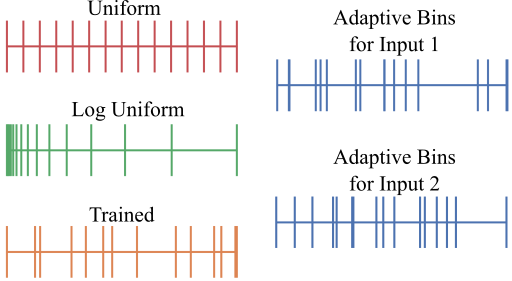
\includegraphics[width=0.7\linewidth]{./figure/bin-types-v2}
   \caption{Choices for bin widths. Uniform and Log-uniform bins are pre-determined. `Trained bins' vary from one dataset to another. Adaptive bins vary for each input image.}
\label{fig:binchoices}
\end{figure}

     第二,将深度间隔 $D$ 离散化为 bin 并将每个像素分配给一个 bin 会导致深度离散化伪影。因此,本文将最终深度预测为 bin 中心的线性组合,使模型能够预测平滑变化的深度值。
     
     第三,几个先前的体系结构提出在网络架构中的编码器块后使用注意力块来进行全局信息处理,当前最先进的深度估计也使用这种策略。这种体系结构由三个按顺序排列的块组成:编码器、注意力,然后是解码器。本文最初遵循这种方法,但注意到在空间分辨率更高的张量上使用注意力可以获得更好的结果。因此,本文提出了一个架构,也有这三个块,但排序如下:编码器,解码器,注意力。
     
    第四,本文希望建立在最简单的架构上,以隔离新提出的 Adabin 概念的影响。因此,本文使用 EfficientNet B5 作为编码器的主干构建了一个编码器-解码器架构的网络。
    
\subsection{架构描述}

 如图 \ref{fig:model} 所示,本文的网络架构由两个主要组件组成:1)建立在预训练的 EfficientNet B5 编码器和标准特征上采样解码器上的编码器-解码器块;2)提出的称为 AdaBins 的自适应 bin 宽度估计器块。
 

\begin{figure*}[!htbp]
\centering
	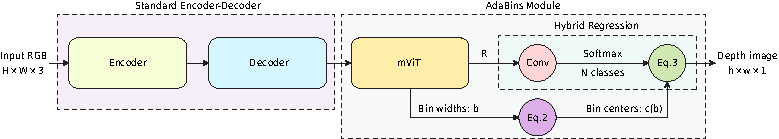
\includegraphics[width=.7\paperwidth]{figure/model}
	\caption{Overview of our proposed network architecture. Our architecture consists of two major components: an encoder- decoder block and our proposed adaptive bin-width estimator block called AdaBins. The input to our network is an RGB image of spatial dimensions H and W , and the output is a single channel h × w depth image (e.g., half the spatial resolution).}
	\label{fig:model}
\end{figure*}

近年来,编码器-解码器这种体系结构的使用在深度估计问题的有监督和无监督两种类别中都显示出巨大的成功。这种方法通常使用一个或多个编码器-解码器网络作为其较大网络的子网络。本文在如图 \ref{fig:model2} 所示结构的基础上进行了修改。这样能够更明确地研究本文提出的扩展在 baseline 上性能提升的归因。

\begin{figure*}[!htbp]
\centering
	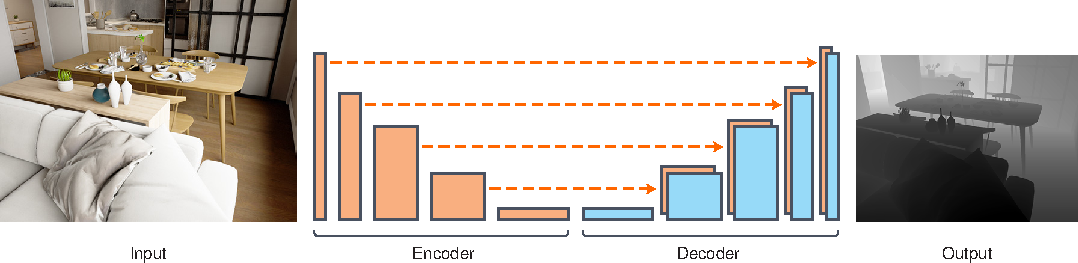
\includegraphics[width=.7\paperwidth]{figure/network_overview}
	\caption{A straightforward encoder-decoder architecture with skip connections. The encoder part is a pre-trained truncated DenseNet-169 with no additional modifications. The decoder is composed of basic blocks of convolutional layers applied on the concatenation of the $2\times$ bilinear upsampling of the previous block with the block in the encoder with the same spatial size after upsampling. }
	\label{fig:model2}
\end{figure*}

所进行的修改是将编码器从 DenseNet 切换到 EfficientNet B5,并为新架构使用适当的损失函数。此外,解码器的输出是张量 $\textbf{x}_d \in \mathbb{R}^{h \times w \times C_d}$,而不是代表最终深度值的单通道图像,此张量被称为“解码特征”。,并作为第二部分 AdaBins 模块的输入,而 AdaBins 模块的输出为大小为 $h \times w \times C_d$ 的张量。由于 GPU 和内存的限制,$h=H/2$,$w=W/2$,最后的深度图通过简单的双边上采样来计算得到与输入图像相同大小。


Transformer 在 NLP 任务和计算机视觉任务中的传统用途之外,正受到越来越多的关注。随着最近将 CNN 与 Transformer 相结合趋势的成功,本文提出利用 Transformer 编码器作为对 CNN 输出进行全局分析的模块,即图 \ref{fig:model} 中所示的 AdaBins 模块。

AdaBins 模块中的第一个块叫做 mini-ViT,如图 \ref{fig:vit} 所示。这是最近提出的一种使用 Transformer 进行图像识别技术的简化版本,mini-ViT有两个输出:1)bin 宽度的向量 $\textbf{b}$,它定义了如何为输入图像划分深度间隔 $D$,以及2)大小为 $h \times w \times C$ 的范围注意力图 $\mathcal{R}$,它包含用于像素级深度计算的有用信息。

\begin{table}[!htbp]
\centering
\caption{Mini-ViT architecture details.}
\setlength{\tabcolsep}{7.5mm}{
\begin{tabular}{@{}lllllll@{}}
\toprule
\begin{tabular}[c]{@{}l@{}}Patch \\ size ($p$)\end{tabular} & E   & Layers & \begin{tabular}[c]{@{}l@{}}num\\ heads\end{tabular} & C   & \begin{tabular}[c]{@{}l@{}}MLP \\ Size\end{tabular} & Params \\ \midrule
16    & 128 & 4      & 4    & 128 & 1024      & 5.8 M \\ \bottomrule
\end{tabular}}
\label{tab:arch-mvit}
\end{table}


\begin{figure*}[!htbp]
\centering
	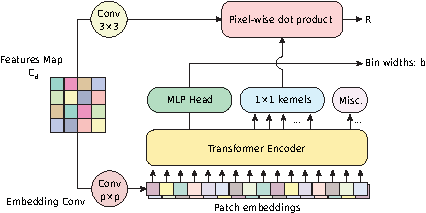
\includegraphics[width=.7\paperwidth]{figure/mViT_v6}
	\caption{An overview of the mini-ViT block. The input to the block is a multi-channel feature map of the input image. The block includes a Transformer encoder that is applied on patch embeddings of the input for the purpose of learning to estimate bin widths $b$ and a set of convolutional kernels needed to compute our Range-Attention-Maps $R$.}
	\label{fig:vit}
\end{figure*}

\subsection{Mini-ViT}

对于给定的图像,估计其深度范围 $D$ 内更可能出现的子间隔需要同时结合局部结构信息和全局分布信息。本文提出使用全局注意力来计算每个输入图像的 bin 宽度向量 $\textbf{b}$。无论是内存还是计算复杂度,全局注意力都是很“昂贵”的,尤其是在较高的分辨率下。然而,最近 Transformer 的快速发展提供了一些有效的替代方案。本文在设计基于 Transformer 的 AdaBins 模块时,从视觉 Transformer (ViT) 中获得了灵感。由于本文使用的数据集更小,因而使用了一个更小版本的 Transformer 编码器,即 mini-ViT 或 mViT,其参数如表 \ref{tab:arch-mvit} 所示。

\subsection{Mini-ViT}

mViT 的输入是解码特征 $\mathbf{x_d}\in~\mathbb{R}^{h \times w \times C_d}$ 的张量。然而,Transformer 以一系列固定大小的向量作为输入。首先将解码后的特征通过一个称为 \textit{Embedding Conv} 的卷积块(如图 \ref{fig:vit} 所示),其卷积核大小为 $p\times p$,步长为 $p$,输出通道数为 $E$。因此,该卷积的结果是大小为 $h/p~\times~w/p~\times E$ 的张量(假设 $h$ 和 $w$ 都可以被 $p$ 整除)。结果被重新排列为空间展平张量 $\mathbf{x_p}~\in~\mathbb{R}^{S\times E}$,$S=\frac{hw}{p^2}$ 作为 Transformer 的有效序列长度,称这个 $E$ 维向量的序列为 \textit{patch embeddings}。

按照通常的做法,本文将学习到的位置编码添加到 patch 嵌入中,然后将它们馈送给 Transformer 并输出一系列输出嵌入 $\mathbf{x_o}~\in~\mathbb{R}^{S\times E}$。在第一个输出嵌入上使用 MLP 头。MLP 头使用一个 ReLU 激活函数并输出一个 N 维向量 $\textbf{b}'$。最后,对向量 $\textbf{b}'$ 进行归一化处理,使其总和为1,从而获得 bin 宽度向量 $\textbf{b}$。归一化在 bin 宽度之间引入了竞争,并迫使网络通过在 $D$ 的兴趣区域预测较小的 bin 宽度来关注 $D$ 内的子间隔。

\begin{equation}
    b_i = \frac{b'_i + \epsilon}{\sum_{j=1}^{N} (b'_j + \epsilon)},
\end{equation}
其中 $\epsilon=10^{-3}$

\subsubsection{Range attention maps}

解码特征表示高分辨率的、局部的像素级信息,而 Transformer 输出的嵌入有效地包含了更多的全局信息。如图 \ref{fig:vit} 所示,来自 Transformer 的输出嵌入 2 到 C + 1 被用作一组 $1 \times 1$ 卷积核,并与解码特征(在 $3\times 3$ 卷积层之后)进行卷积,以获得范围-注意力图 $\mathcal{R}$。这相当于计算被视为“key”的像素级特征和被视为“query”的 Transformer 输出嵌入之间的点积注意力权重。这种使用输出嵌入作为卷积核的简单设计使得网络将自适应全局 Transformer 集成到解码特征的局部信息中。$\mathcal{R}$ 和 $\textbf{b}$ 一起用来获得最终的深度图。

范围-注意力图 $\mathcal{R}$ 通过 $1 \times 1$ 卷积和一层 Softmax 来调整得到 $N$ 个通道。$N$ Softmax 分数 $p_k$ 被解释为每个像素位于 $N$ 个深度 bin 中心的概率 $c(\textbf{b}) := \{c(b_1), c(b_2), ..., c(b_N)\}$,由 bin 宽向量 $\textbf{b}$ 计算得:

\begin{equation}
    c(b_i) =  d_{min} + (d_{max} - d_{min})(b_i/2 + \sum_{j=1}^{i-1} b_j)
\end{equation}

每个像素的最终深度值 $\Tilde{d}$ 由该像素处的 Softmax 分数和深度 bin 中心 $c(\textbf{b})$ 的线性组合计算得到。

\begin{equation}
    \Tilde{d} = \sum_{k=1}^N c(b_k) p_k
\end{equation}

\section{Experiments}
\label{experimentes}

以 NYU Depth v2 数据集为例,该数据集包含 120K 个训练样本和 654 个测试样本。本文在一个 50K 的子集上进行训练。网络输出分辨率为 $320 \times 240$ 的深度预测,然后将其上进行 $2 \times$ 采样以在训练和测试期间匹配真值的分辨率。在测试时,通过取图像预测和镜像预测的平均值来计算最终输出,这是之前工作的常用方法。

性能对比如表 \ref{tab:results-nyu} 所示。虽然 NYU 的最先进性能已经停滞了相当长的一段时间,但本文的方法能够在所有指标上显着超越最先进的性能。

在消融实验中,首先评估了 AdaBins 模块的重要性。作者从架构中移除了 AdaBins 模块,并使用编码器-解码器通过设置 $C_d=1$ 直接预测深度图,并将其与 AdaBins 模块的变体进行比较。如表 \ref{tab:ablation-arch} 显示,没有 AdaBins 的架构(第 1 行)的性能比所有其他变体(第 2-5 行)差。而在 bin 设计的选择上,Trained-but-Fixed 变体在所有选择中表现最差,本文使用的自适应 bin 的最终选择显着提高了性能并优于所有其他变体。

\begin{table}[!htbp]
\centering
\setlength{\tabcolsep}{7mm}{
%\begin{adjustbox}{width=0.5\linewidth}
\begin{tabular}{@{}llllll@{}}
\toprule
\textbf{Variant}        & \textbf{$\delta_1$}$\uparrow$       & \textbf{$\delta_2$}$\uparrow$          & \textbf{$\delta_3$}~$\uparrow$            & REL~$\downarrow$          & RMS~$\downarrow$ \\ \midrule
Base + R          & 0.881          & 0.980          & 0.996          & 0.111            & 0.419                 \\
Base + Uniform-Fix-HR                         & 0.892          & 0.981          & 0.995          & 0.107            & 0.383                \\
\begin{tabular}[c]{@{}l@{}}Base + Log-Fix-HR\end{tabular} & 0.896          & 0.981          & 0.995          & 0.108            & 0.379                  \\
\begin{tabular}[c]{@{}l@{}}Base + Train-Fix-HR\end{tabular}     & 0.893          & 0.981          & 0.995          & 0.109            & 0.381                \\
\textbf{Base + AdaBins-HR}                                                                 & \textbf{0.903} & \textbf{0.984} & \textbf{0.997} & \textbf{0.103}   & \textbf{0.364} \\
\bottomrule
\end{tabular}}
%\end{adjustbox}
\caption{Comparison of different design choices for bin-widths and regression. AdaBins module results in a significant boost in performance. Base: encoder-decoder with an EfficientNet B5 encoder. R: standard regression. HR: Hybrid Regression. (Log)Uniform-Fix: Fixed (log) uniform bin-widths. Train-Fix: Trained bin-widths but Fixed for each dataset.}
\label{tab:ablation-arch}
\end{table}


\begin{table*}[!htbp]
\centering
\caption{Comparison of performances on the NYU-Depth-v2 dataset. The reported numbers are from the corresponding original papers. Best results are in bold, second best are underlined.}
\begin{tabularx}{\linewidth}{@{}l*{5}{C}c@{}}
\toprule
Method        & \textbf{$\delta_1$}$\uparrow$       & \textbf{$\delta_2$}$\uparrow$          & \textbf{$\delta_3$}~$\uparrow$            & REL~$\downarrow$          & RMS~$\downarrow$  & $log_{10}$~$\downarrow$ \\ \midrule
Eigen                                                       & 0.769          & 0.950          & 0.988          & 0.158            & 0.641          & --              \\ 
Laina                                                   & 0.811          & 0.953          & 0.988          & 0.127            & 0.573          & 0.055                \\ 
 MS-CRF                                                             & 0.811          & 0.954          & 0.987          & 0.121            & 0.586          & 0.052          \\ 
Hao~\etal                                                     & 0.841          & 0.966          & 0.991          & 0.127            & 0.555          & 0.053                \\ 
Lee~\etal                                                    & 0.837          & 0.971          & 0.994          & 0.131            & 0.538          &   --                   \\
Fu~\etal                                                     & 0.828          & 0.965          & 0.992          & 0.115            & 0.509          &   0.051                   \\
SharpNet                                                            & 0.836          & 0.966          & 0.993          & 0.139            & 0.502          &      \underline{0.047}          \\
% Alhashim~\etal~\cite{Alhashim2018}                                                            & 0.846          & 0.974          & 0.994          & 0.123            & 0.465          &      0.053          \\
Hu~\etal                                                               & 0.866          & 0.975          & 0.993          & 0.115            & 0.530          &    0.050            \\ 
Chen~\etal                                                      & 0.878          & 0.977          & 0.994          & 0.111            & 0.514          &  0.048              \\ 
Yin~\etal                                                             & 0.875          & 0.976          & 0.994          & \underline{0.108}            & 0.416          & 0.048               \\ 
BTS~                                                              & \underline{0.885}          & 0.978          & 0.994          & 0.110            & \underline{0.392}          & \underline{0.047}          \\ 
DAV                                                              & 0.882          & \underline{0.980}          & \underline{0.996} & \underline{0.108}            & 0.412          & --              \\ 
\midrule

\textbf{AdaBins (Ours)} & \textbf{0.903} & \textbf{0.984} & \textbf{0.997} & \textbf{0.103}     & \textbf{0.364} & \textbf{0.044} \\ 
\bottomrule
\end{tabularx}
\label{tab:results-nyu}
\end{table*}

\begin{figure*}[!htbp]
     \centering
     \subcaptionbox{RGB}{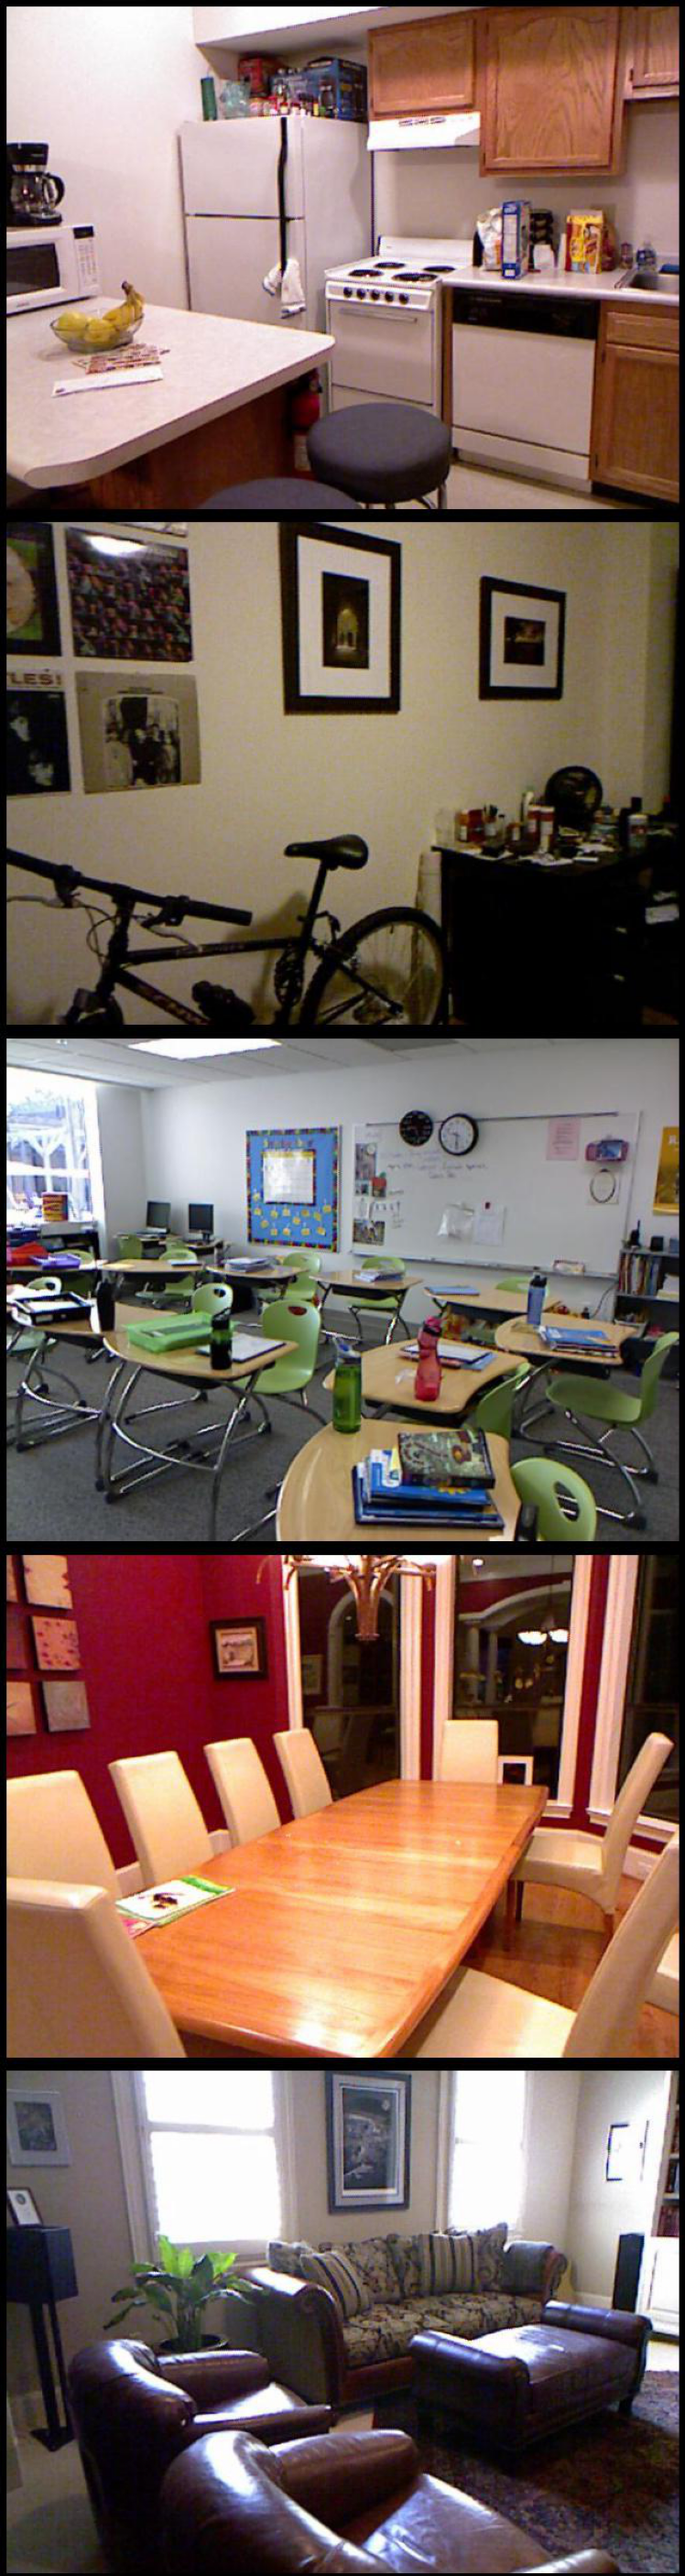
\includegraphics[height=10.5cm]{./figure/RGB.png}}\hspace{0.3em}%
     \subcaptionbox{BTS}{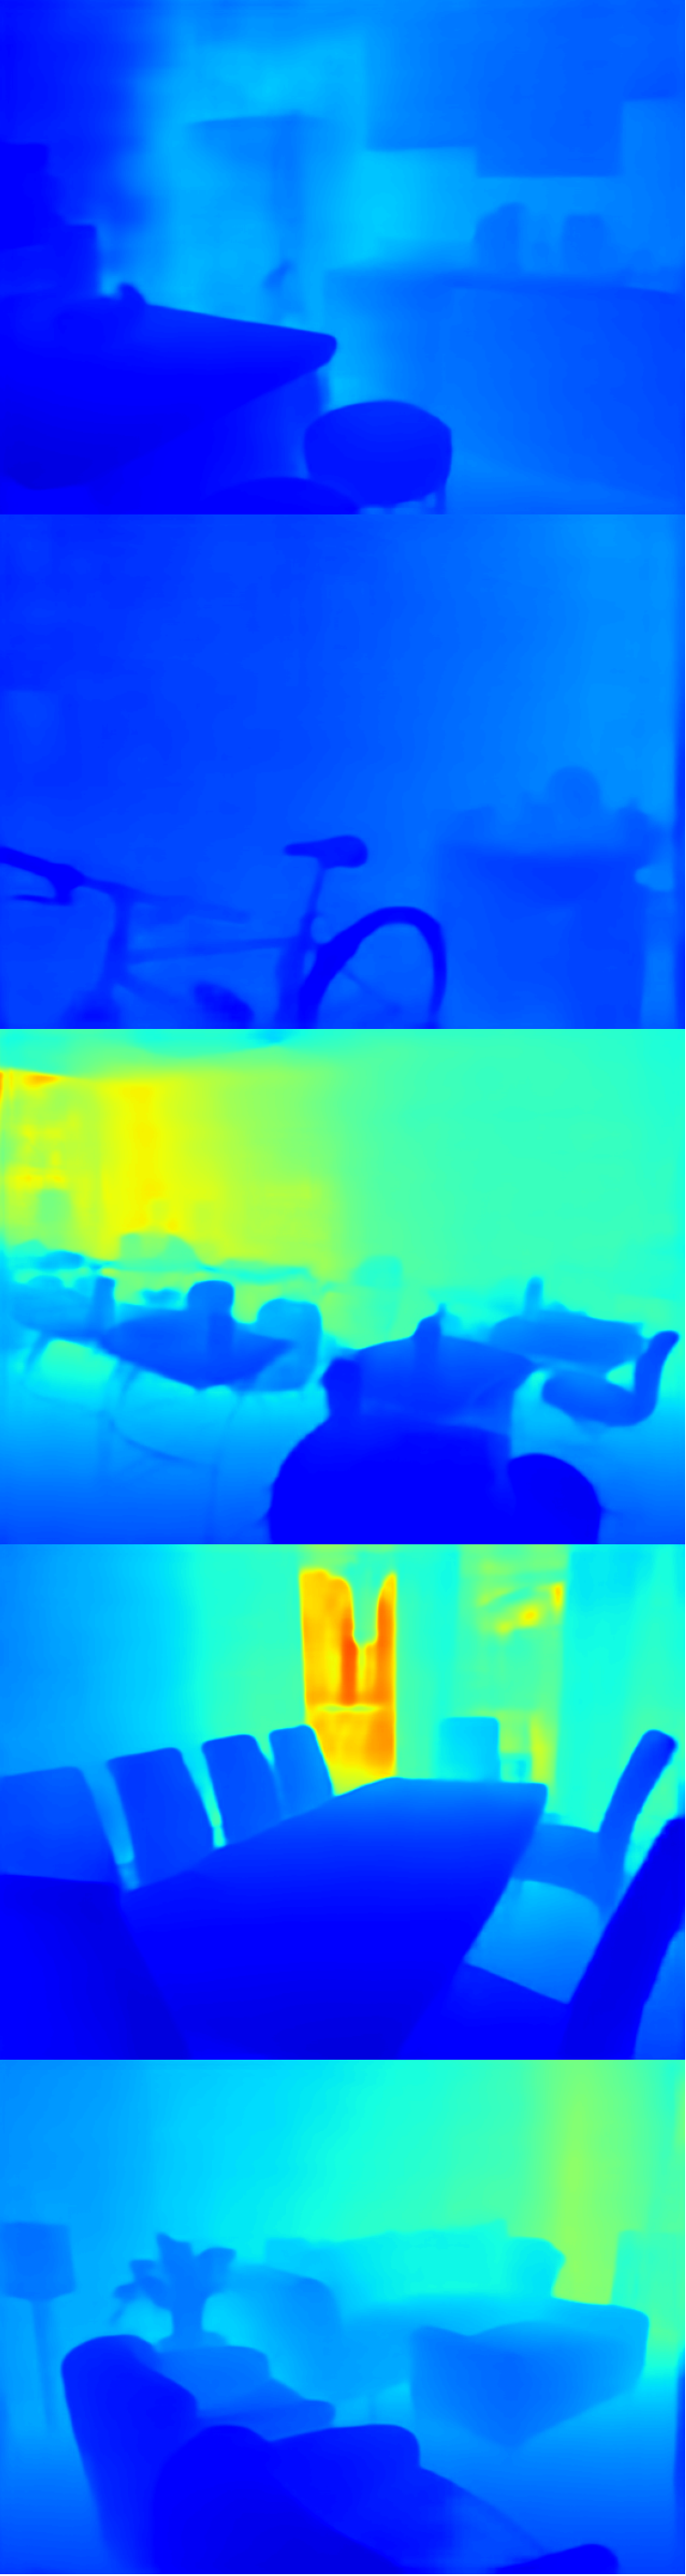
\includegraphics[height=10.5cm]{./figure/BTS.png}}\hspace{0.3em}%
     \subcaptionbox{DAV}{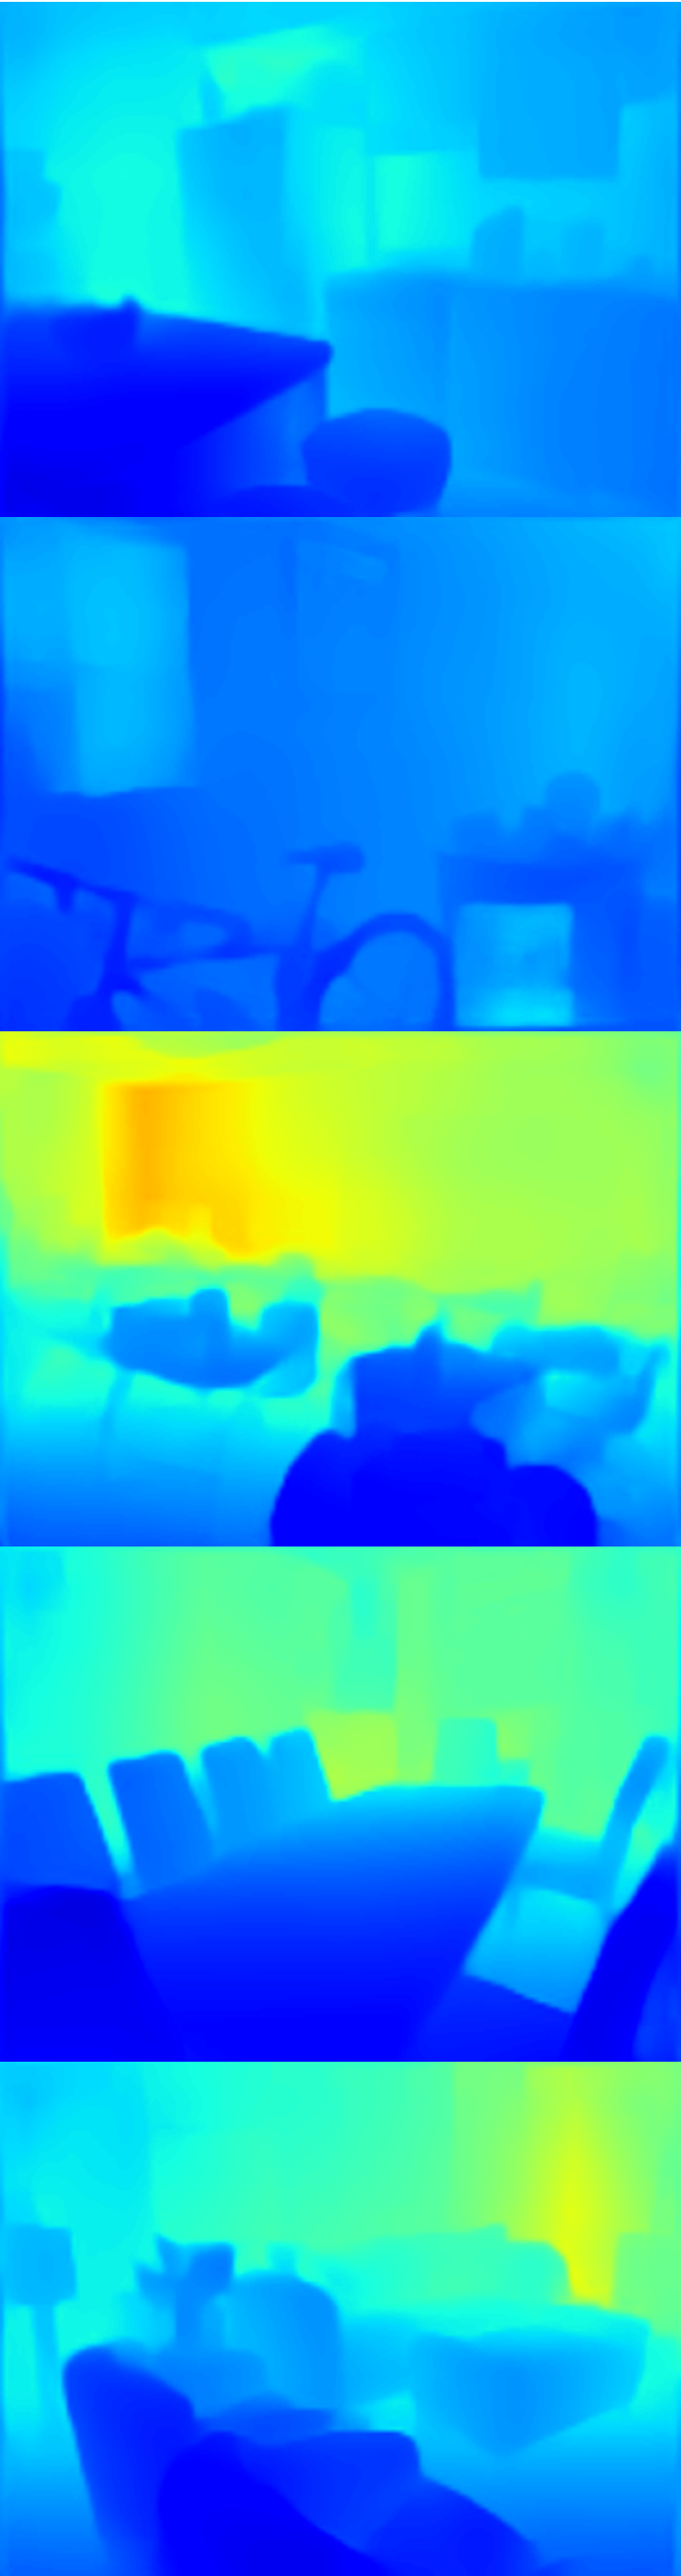
\includegraphics[height=10.5cm]{./figure/DAV.png}}\hspace{0.3em}%
     \subcaptionbox{Ours}{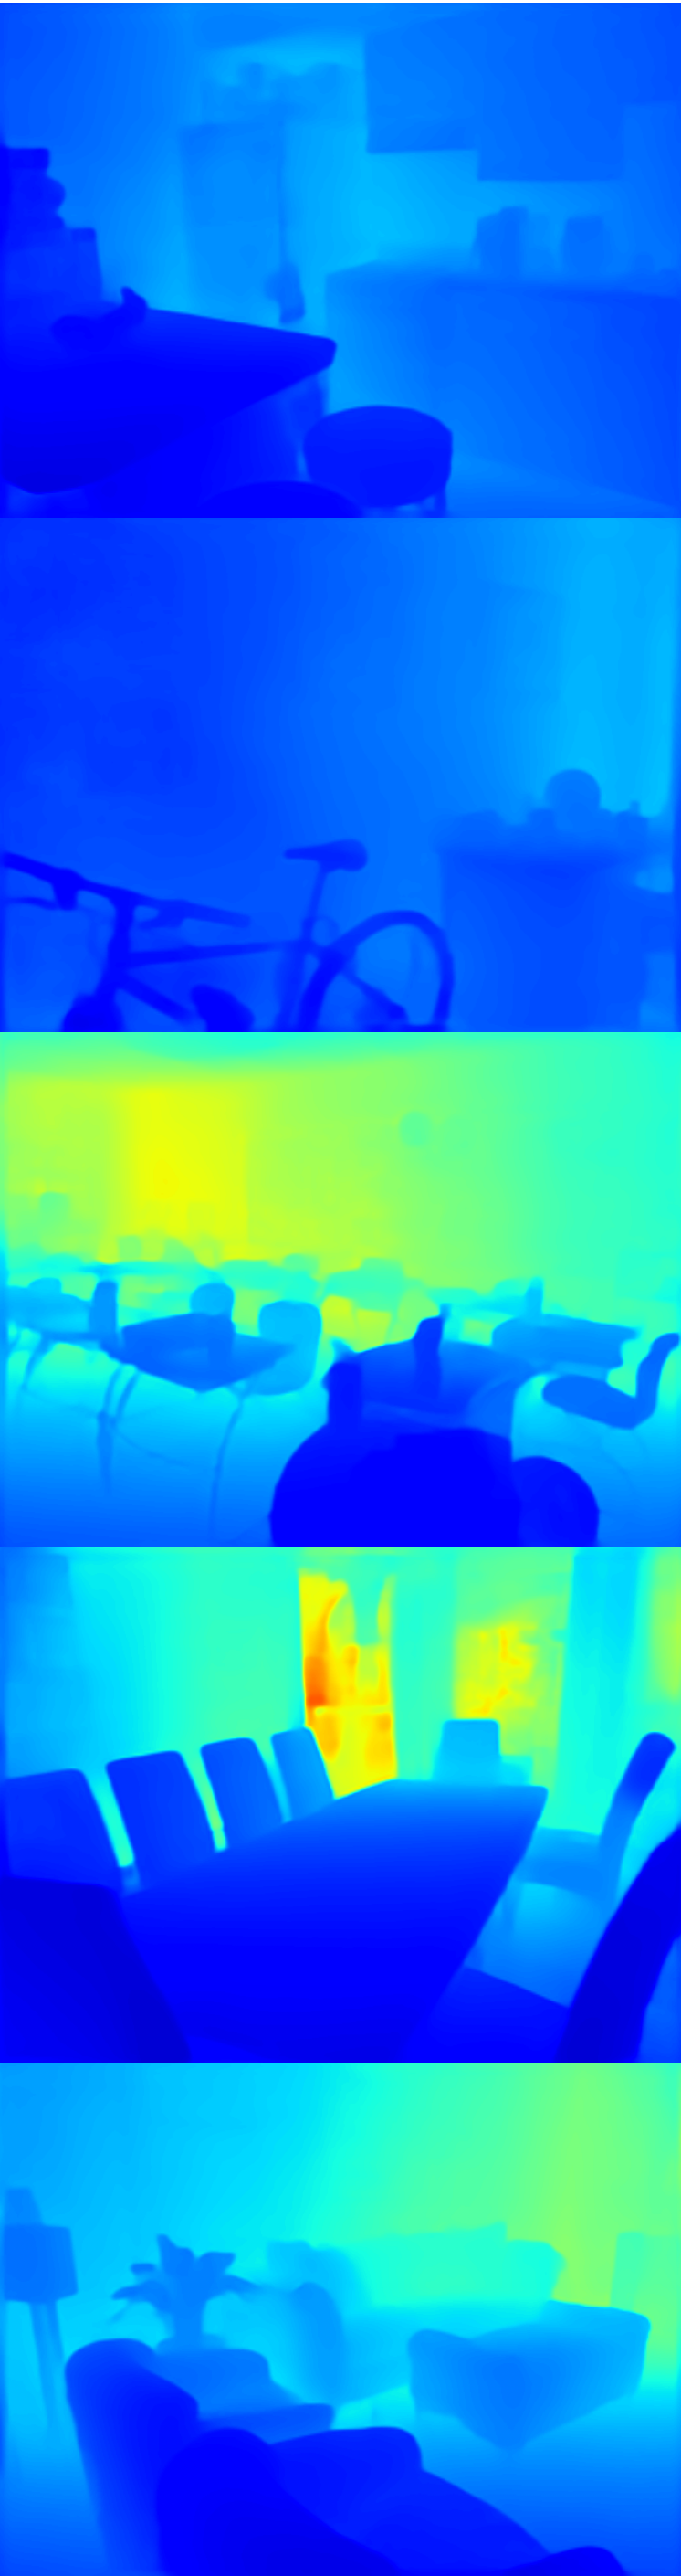
\includegraphics[height=10.5cm]{./figure/OURS.png}}\hspace{0.3em}%
     \subcaptionbox{GT}{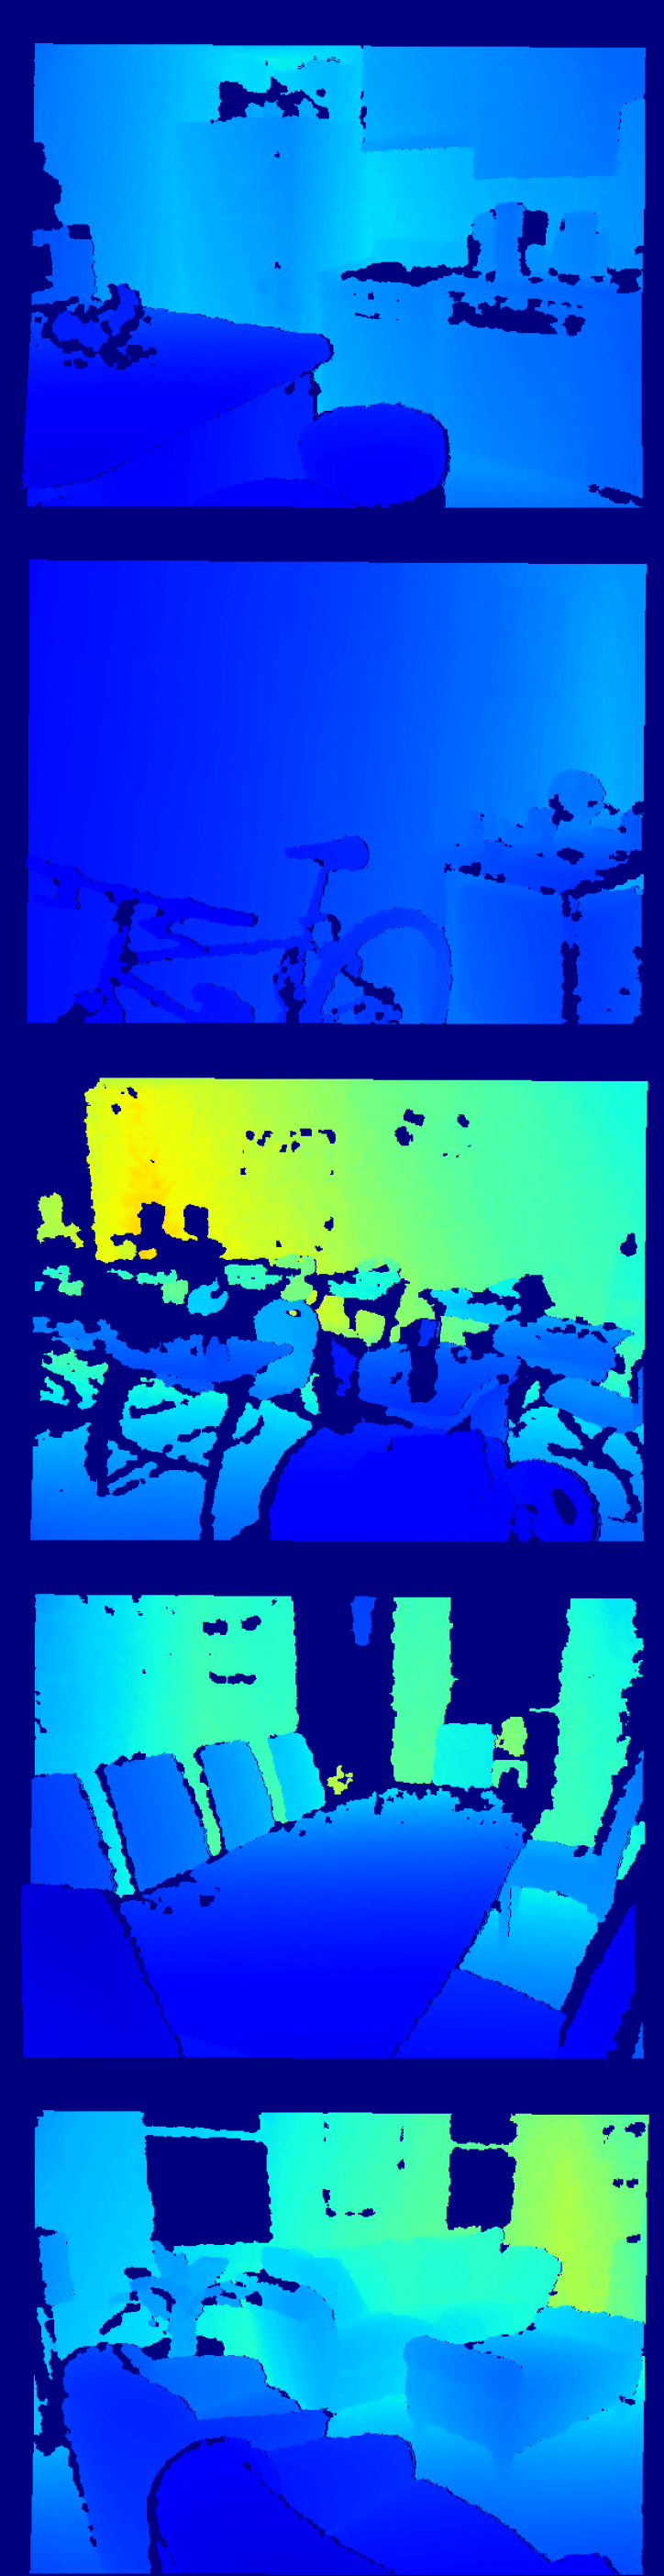
\includegraphics[height=10.5cm]{./figure/GT.png}}
        \caption{Qualitative comparison with the state-of-the-art on the NYU-Depth-v2 dataset.}
        \label{fig:qualitative-comparison}
\end{figure*}



%\begin{lstlisting}
%# \lstinputlisting{code/demo.py}
%import torch
%import torch.nn as nn
%
%print("pytorch")
%\end{lstlisting}

\end{document}
